\section{Trust Region Policy Optimization (TRPO)}
\begin{frame}{}
    \LARGE Policy Search: \textbf{Trust Region Policy Optimization (TRPO)}
\end{frame}

\begin{frame}{Trust Region Policy Optimization (TRPO)}
\begin{itemize}
    \item TRPO updates policies by taking the largest step possible to improve performance, while satisfying a special constraint on how close the new and old policies are allowed to be.
    \item The constraint is expressed in terms of KL-Divergence
    \item This is different from normal policy gradient, which keeps new and old policies close in parameter space
    \item TRPO nicely avoids this kind of collapse, and tends to quickly and monotonically improve performance
    \item TRPO uses conjugate gradients for computing the hessian matrix for KL divergence derivative
\end{itemize}

\footnotetext{https://spinningup.openai.com/en/latest/algorithms/trpo.html}
    
\end{frame}

\begin{frame}{Trust Region Policy Optimization (TRPO)}
\begin{itemize}
    \item TRPO uses backtracking line search with exponential decay (decay coeff $\alpha \in (0, 1)$, budget L) to make appropriate step sizes
    
\end{itemize}

\begin{figure}
\centering
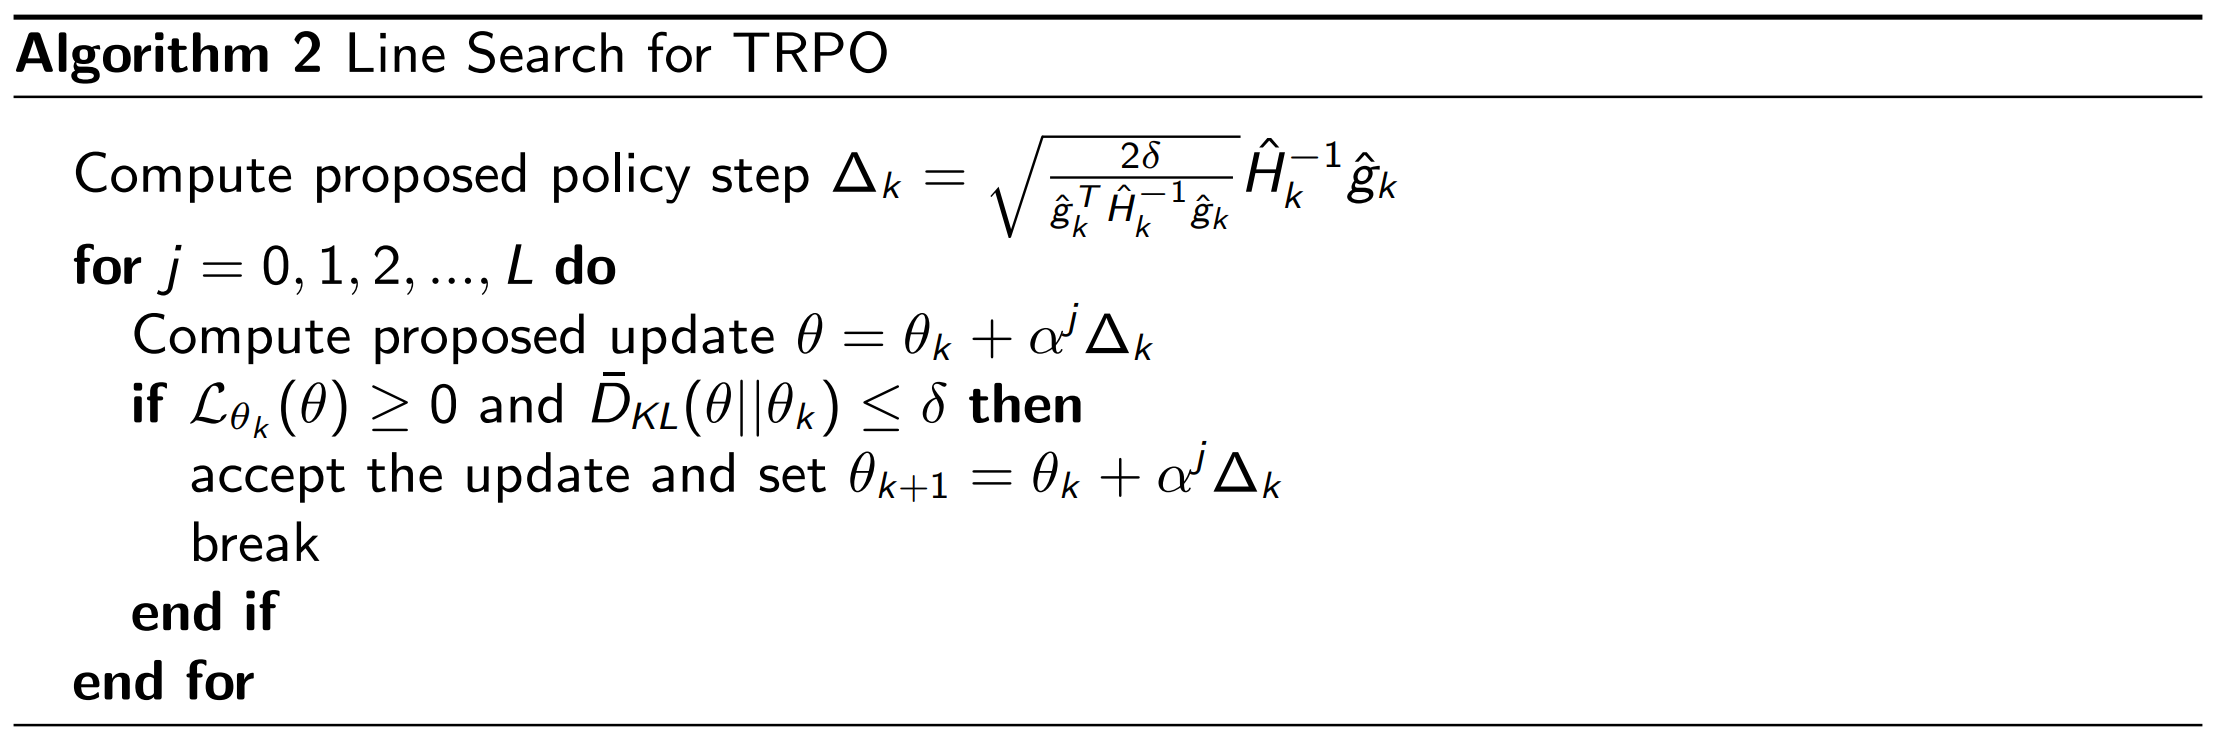
\includegraphics[width=0.9\textwidth,height=0.6\textheight,keepaspectratio]{images/policy-search/trpo_1.png}
\end{figure}
    
\end{frame}

\begin{frame}{Trust Region Policy Optimization (TRPO)}
\begin{figure}
\centering
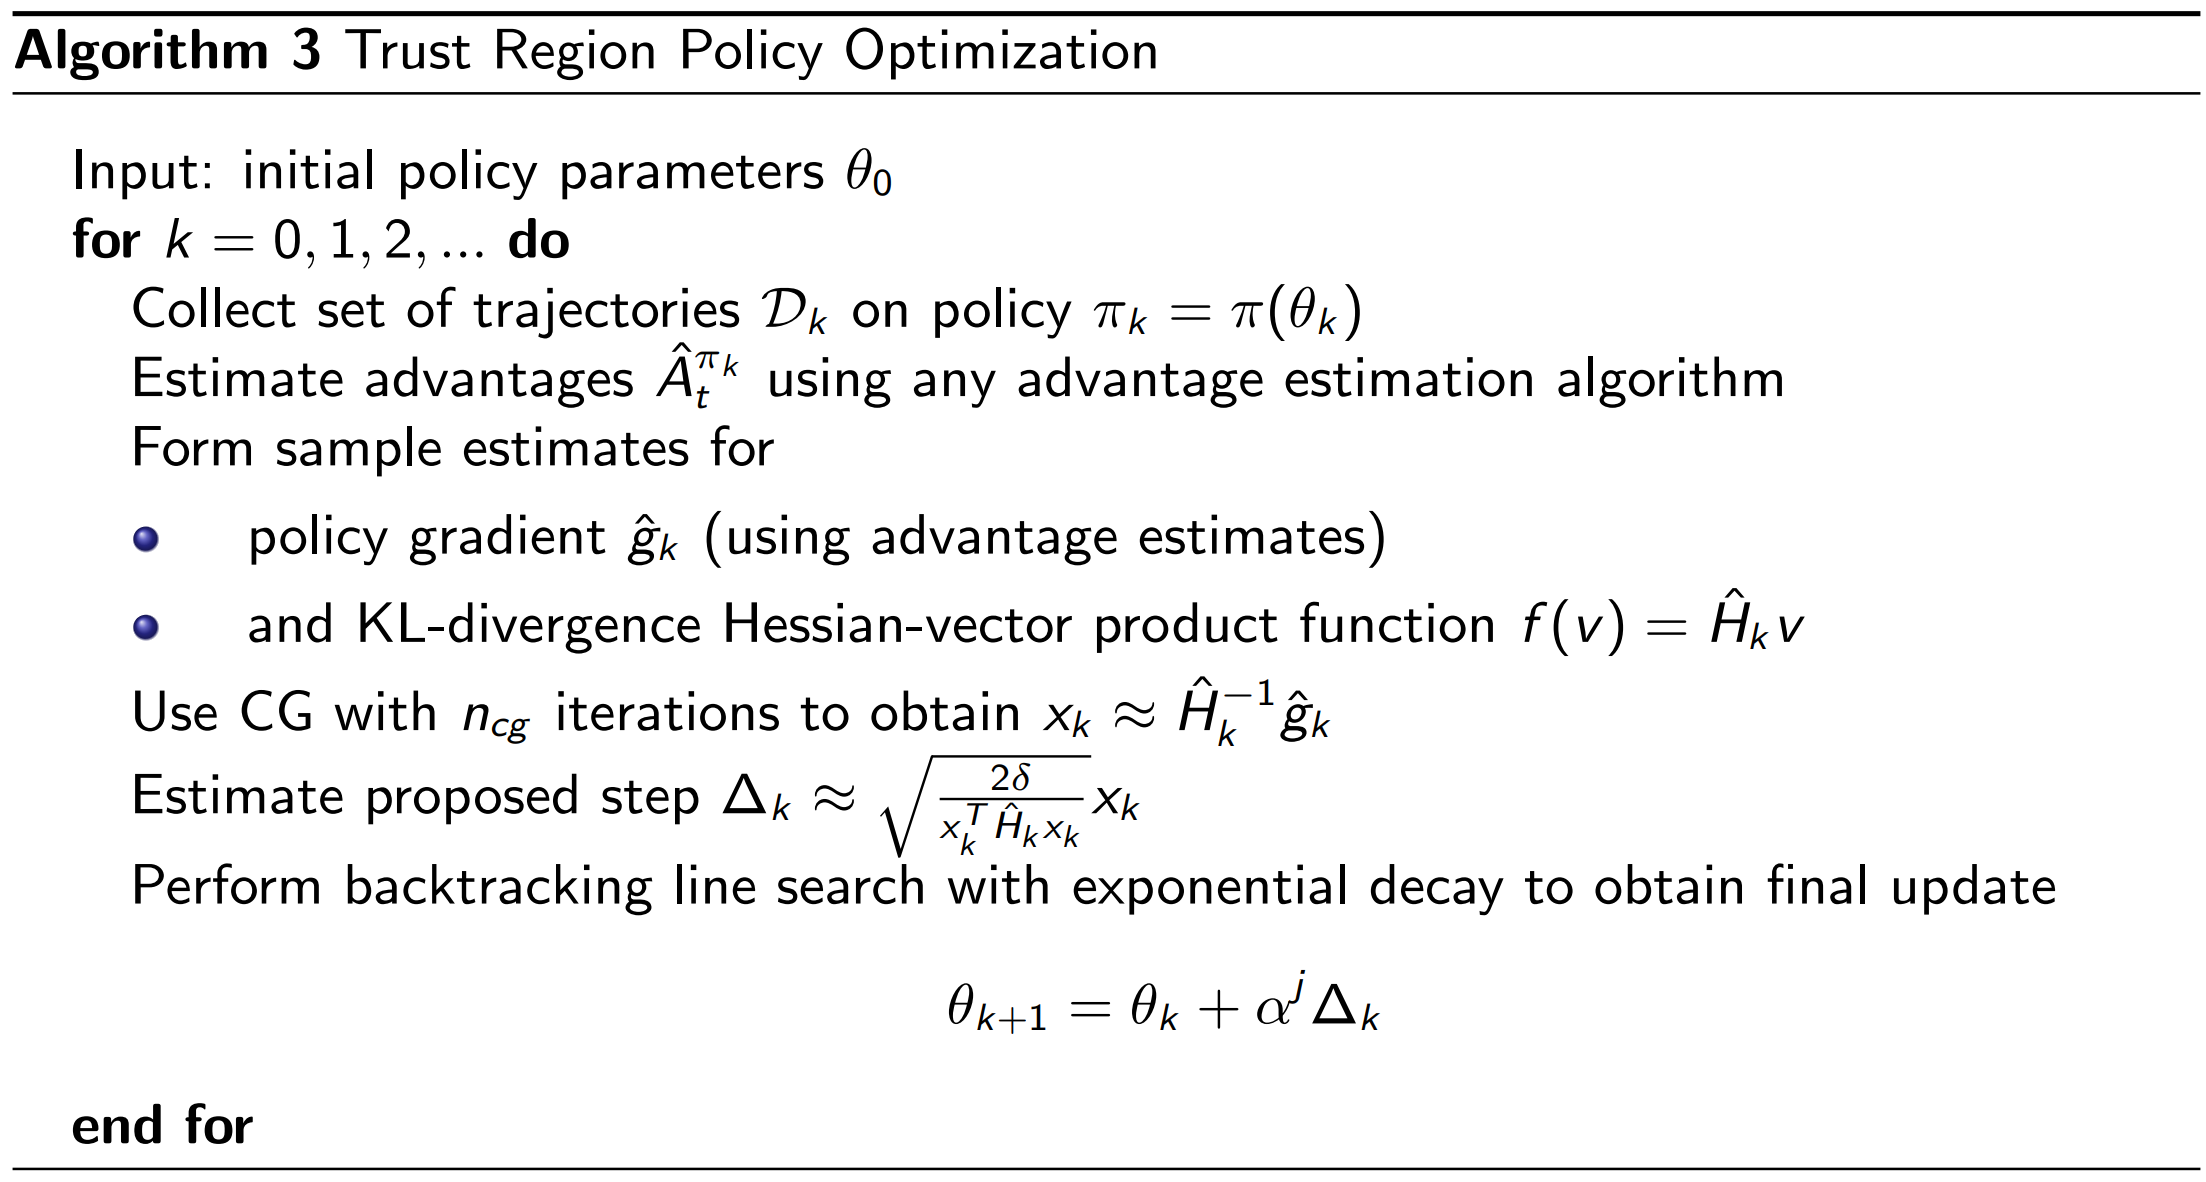
\includegraphics[width=0.9\textwidth,height=0.9\textheight,keepaspectratio]{images/policy-search/trpo_2.png}
\end{figure}
    
\end{frame}